% !TEX root = ../thesis.tex

\chapter{Modelling motion on the \textsc{er}}\label{sec:modelling}

The messy behaviour of Aβ molecules we saw in \cref{sec:data_analysis} by the analysis of \tsc{SPT} data suggests a new hypothesis. The complex and delocalised dynamics that we found may involve active transport on the \emph{endoplasmic reticulum}, a network like organelle supporting various functions encompassing protein folding and redistribution. While it is known that the \tsc{ER} is acts as an active transportation network, it is not possible to find a directionality and the dynamics of such transport mechanism remains not clear \cit{nehls2000dynamics}.
In a recent work, Holcman's team\cit{holcman2018single} has shown that particles moving on the \tsc{ER} follow a two-state process, characterised by alternation of a high-velocity directed motion state associated to flow in the network tubules and a low-velocity diffusing state associated to the nodes. This kind of behaviour, with particles jumping between areas of slow motion, resembles the results the analysis performed in \cref{sec:full_picture}, motivating the hypothesis that transport of Aβ is linked to the \tsc{ER}.

As the inner workings of the \tsc{ER} are not known, it would be difficult to directly compare the the results of \cref{sec:data_analysis} to the \tsc{ER} dynamics. How are molecules redistributed in the \textsc{er}? Which timescale characterise this transport process? First, we have to understand how this network works. Thus, in this chapter we make a step back and we focus on a model of motion on the \tsc{ER}, building on the results of previous analysis, \cit{holcman2018single} and presenting results of numerical simulations to understand the model characteristics.

\begin{figure}[t!]
  \sidecaption{The endoplasmic reticulum of a \tsc{HEK 293T} cell imaged by fast SIM.\label{fig:er}}
  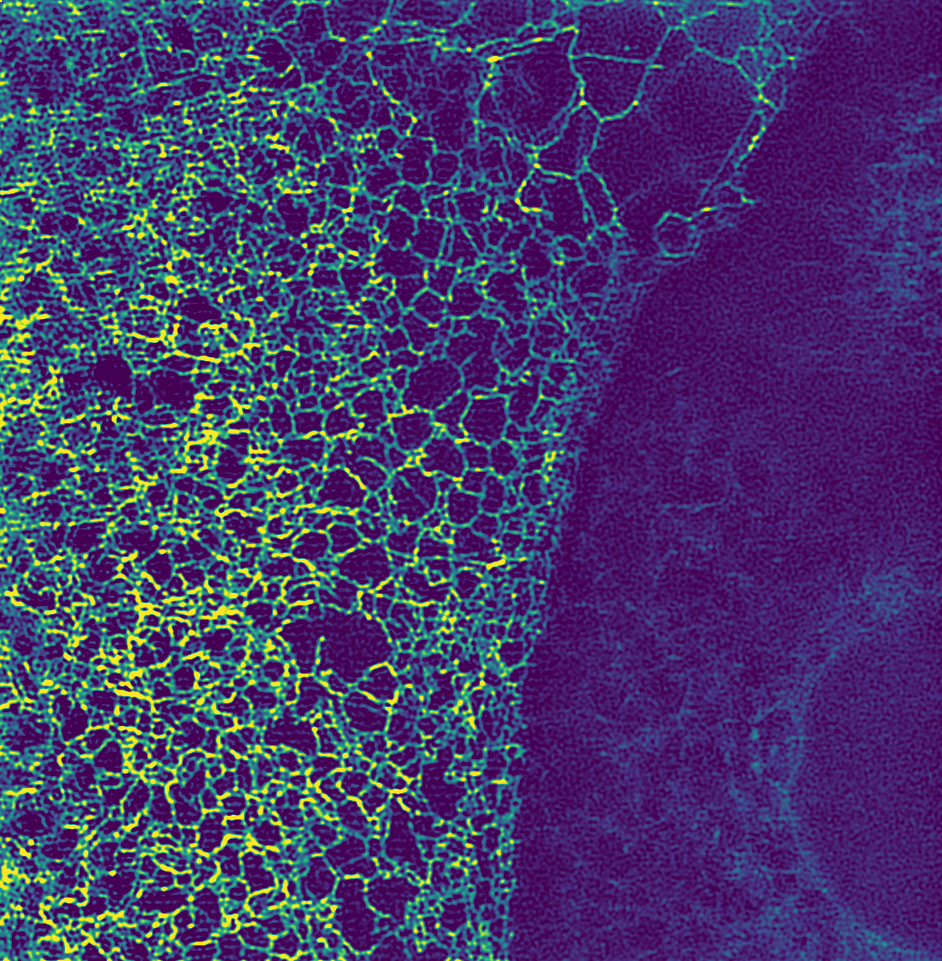
\includegraphics[width=\textwidth]{er.png}
\end{figure}

\section{Active network model}

The \textsc{er} is an organelle that spans from the nuclear envelope to the cell periphery. It has a fundamental role in the production, maturation and trafficking of proteins and lipids. A recent study based on super resolution imaging \cit{ls_er} has revealed hat its structure is made almost exclusively of tubules at varying densities. The tubules are usually connected by three-way junctions at roughly 120 degrees \cit{terasaki1986microtubules} (see also \cref{fig:er}). Since we only have 2 dimensional images we will refer to a planar representation of the \tsc{ER} network. This approximation is jutified by the fact that in many kind of cells the \tsc{ER} is very thin with respect to its width. Given its regular three-way junctions, the simpler planar graph representing the \tsc{ER} is an hexagonal lattice.

Some characteristics of motion on the \tsc{ER} has been recently described through the analysis of \tsc{SPT} trajectories \cit{holcman2018single}. First, luminal proteins follow distinct transport mechanisms depending on topology: they move at fast velocity along the network tubules, and they instead move with dominant diffusive component while inside the junctions. Moreover, the luminal flow along tubules was observed to invert its direction at random time, possibly due to tubule constrictions. We introduce a model of motion that takes into account these effects.

We consider a transported molecule as a random walker on a directed graph, where edges invert their direction at a Poissonian rate ($\lambda$). Each edge will keep a directionality for an exponential time (timescale $\tau_{switch} = \frac{1}{\lambda}$), then reverse it, and so on and so forth. Moreover, the random walker spends an exponential time in each node (with timescale $\tau_{node}$). This takes into account the time required to escape from a node, given the diffusive motion inside the junction\cit{net}. After the waiting in the node, the walker jumps randomly through one of the available outward directed edges and continues its travel. If all the edges happen to be directed inwards, the particle cannot escape and has to wait another exponential time in the node. An example of the network model is shown in figure \ref{fig:model}

\begin{figure}
  \sidecaption{Active network model. Particles diffuse inside the junctions and quickly jump along the edges. The direction of the edges alternates with rate $\lambda$ and the particles take an exponential time to escape from a junction by Brownian motion (timescale $\tau_{node}$). A trapped state (no outward flux from a junction) is marked by the dashed red rectangle.\label{fig:model}}
  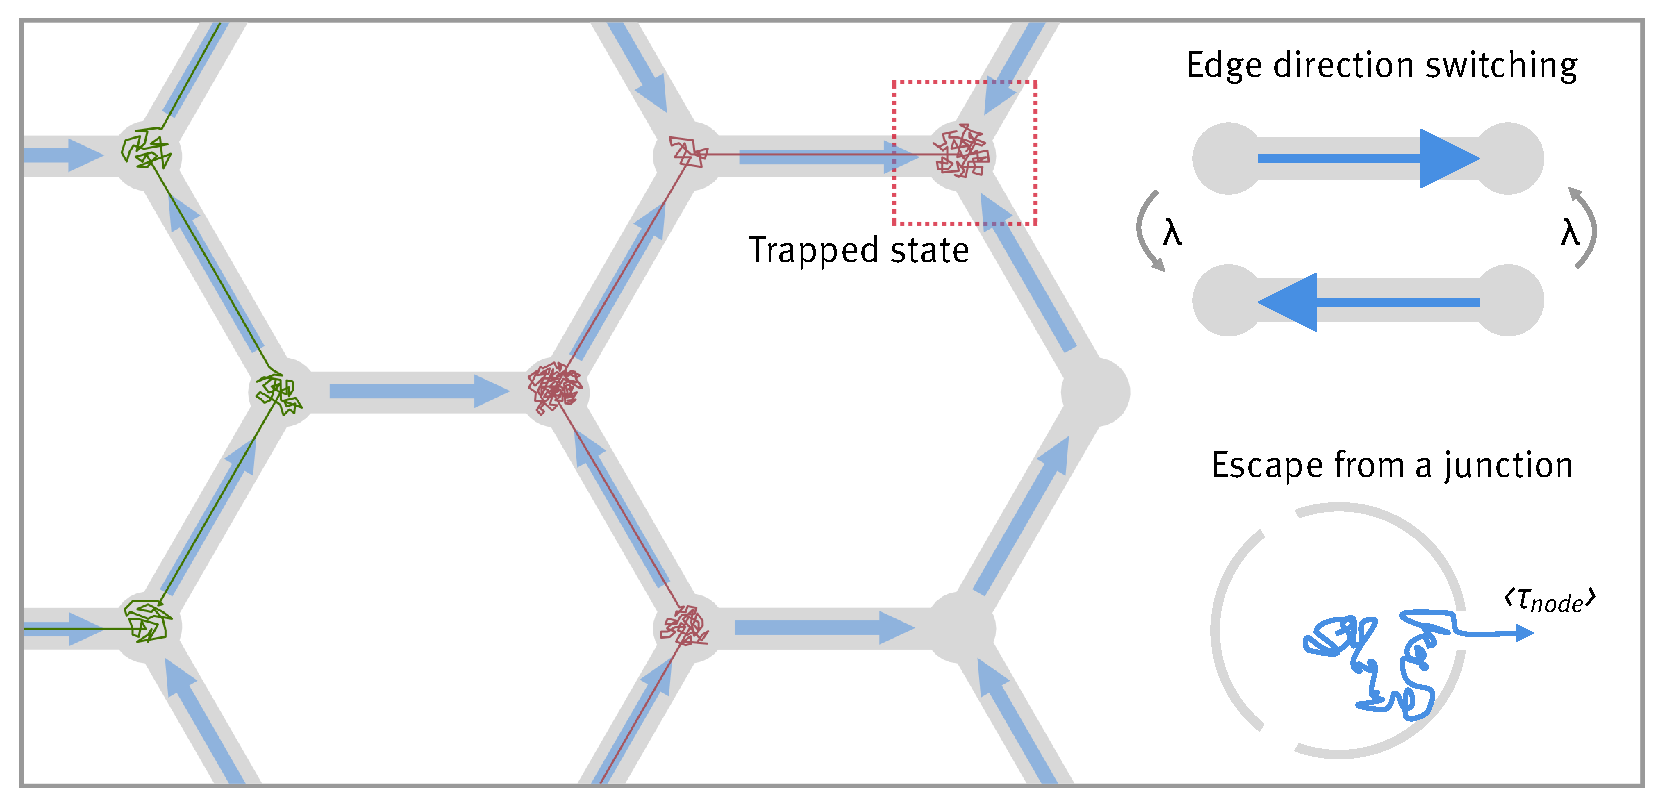
\includegraphics[width=\textwidth]{er/3_model.eps}
\end{figure}

\section{Timescale of transport}

We evaluate now the timescale of the transport on an active network. We consider two timescales that have important biological implications: the mean first passage time (\tsc{mfpt}) through a given node for a single particle and the average time required for the first particle of a group to reach a given node. This second case models an activation process where many particles are released from a source but one is sufficient to activate a receptor located in a far away node.

\subsection{Mean first passage time}

Considering a particle moving on graph starting from node $S$, the \emph{first passage time} (or \emph{hitting time}) for node $T$ is the time at which the particle first hits the target $T$. More formally,
\begin{equation}
  \tau_{S \to T}(x) = \inf \left\{ t: x(t) = T \mid x(0) = S \right\}
\end{equation}
where $x(t)$ denotes the location of the particle at time $t$.
It follows that, if $x(t)$ describes a stochastic motion, we can define the mean first passage time as
\begin{equation}
  \bar{\tau}_{S \to T} = \mathbb{E}_x\left[\tau_{S \to T}(x) \mid x(0) = S\right]
\end{equation}
where the expectation is taken over many realisations of the process.


\subsection{Extreme first passage time}

We now consider the case of $N$ particles moving simultaneously on the network, all starting at the same time from the same source node $S$. In this case, we are interested in knowing the average time required for the first among the $N$ particles to hit the target $T$. Again, this is a common situation in biological systems, where a single particle may be sufficient to activate a receptor (for example, in a synapse). We define this as the minimum hitting time among N independent processes:
\begin{equation}
  \tau^{ex}_{S \to T}(N) = \min \left\{ \tau_{S \to T}(x_1), \tau_{S \to T}(x_2), \dots, \tau_{S \to T}(x_N) \right\}
\end{equation}
We can then take the average over many realisations of this multiple-particle process to define
\begin{equation}
  \bar{\tau}^{ex}_{S \to T}(N) = \mathbb{E}_{\{x_1, x_2, \dots, x_N\}} \left[ \tau^{ex}_{S \to T}(N) \right]
\end{equation}
We name this last quantity \textit{extreme first passage time} (\textsc{efpt}).

\subsection{Numerical simulations and results}

Numerical simulations of the model were performed to measure mean and extreme first passage time on both a synthetic hexagonal lattice and a reconstruction of a real network from \tsc{SIM} imaging data. The model parameters used---unless specified otherwise---are based on the timescales observed in the \tsc{spt} data analysed in \cit{holcman2018single} and are summarized in table \ref{table:sim_params}.


\begin{margintable}
  \sffamily
  \begin{tabular}{@{}ll@{}}
    $\tau_{node}$   & \SI{100}{\milli\second}  \\
    \hline
    $\tau_{switch}$ & \SI{30}{\milli\second}  \\
    \hline
  \end{tabular}
  \caption{Parameters values used for numerical simulations.}\label{table:sim_params}
\end{margintable}

\begin{figure}
  \begin{adjustwidth*}{}{-46mm}
    \includegraphics[width=186mm]{er/3_timescales.eps}%
    {{\phantomsubcaption{}\label{fig:ts_er}}%
    {\phantomsubcaption{}\label{fig:ts_hex}}%
    {\phantomsubcaption{}\label{fig:ts_switching}}}%
    \caption{Timescales in the active network.
    \subref{fig:ts_er}\enspace \tsc{MFPT} (heatmap and distance plot) on the network reconstructed from \tsc{SIM} imaging, \subref{fig:ts_hex}\enspace \tsc{MFPT} on an equivalent hexagonal lattice. Boundary effects are visible at the extremal regions that are weakly connected to the bulk of the network.
    \subref{fig:ts_switching}\enspace effect on the \tsc{MFPT} of the switching timescale $\tau_{switch}$ for $d(S, T) = 25$ for the hexagonal lattice. The red region indicates the range of biologically plausible values of $\tau_{switch}$ taken from \cite{holcman2018single}.\label{fig:ts}}

  \end{adjustwidth*}
\end{figure}

\section{Collective motion}
